\documentclass[a4paper, oneside, twocolumn, 10pt, table]{report}

\usepackage[utf8]{inputenc}
\usepackage{graphicx}
\usepackage{listings}
\usepackage{float}
\usepackage{amsmath}
\usepackage{amssymb}
\usepackage{xparse}
\PassOptionsToPackage{hyphens}{url}\usepackage{hyperref}
\usepackage{cleveref}
\usepackage{enumitem}
\usepackage{algorithm}
\usepackage{algpseudocode}
\usepackage{supertabular}
\usepackage[toc, page]{appendix}
\usepackage{listings}
\usepackage{textcomp}
\usepackage{gensymb}
\usepackage{xcolor}

\lstset{
  basicstyle = \ttfamily\footnotesize,
  keywordstyle = \bfseries,
  breaklines = true,
  postbreak = \mbox{$\hookrightarrow$\space},
  numbers = left,
  stepnumber = 1,
  showstringspaces = false,
}
\renewcommand{\ttdefault}{pcr}
\setlist{parsep = 0pt, listparindent = \parindent}

\crefname{applbl}{appendix}{appendices}
\Crefname{applbl}{Appendix}{Appendices}
\crefname{chplbl}{question}{questions}
\Crefname{chplbl}{Question}{Questions}
\renewcommand{\chaptername}{Question}
\crefalias{chapter}{chplbl}

\title{\bf
  \LARGE [2IMF25] Assignment part 2\\
}
\author{
  Geenen, R. (0843558) \\
  Mols, J. (0851883) \\
}

\begin{document}
\maketitle
\tableofcontents

\chapter{}\label{chp:1}
We completed this question with Z3. To model this question such that Z3 can solve it, we have to create more variables for every step of time. First, we look at the number of pallets loaded in the truck. For every point in time, we create a variable. Let $tp_{\delta}$ denote the amount of pallets in the truck at step $\delta$, where $0 \leq \delta \leq \infty$. For the given situation (in (a)), we initialize $tp_0$ to 300. The truck also has a maximum load, in this case 300. We then have the following constraints:

\begin{equation}
    \label{maxload}
    \bigwedge^{\infty}_{\delta=0} (tp_{\delta} \geq 0 \wedge tp_{\delta} \leq 300)
\end{equation}

Next, we define variables for the amount of food pallets in each village's stock. We let $sb_{x,\delta}$ denote the amount of pallets in stock at village $x$, at step $\delta$, \textit{before} delivery, where $x \in V$ is a village in the given set of villages $V$ that need food. Similarly, we also have $sa_{x,\delta}$ denote the amount of pallets in stock at village $x$, at step $\delta$, \textit{after} delivery. We want the villages to always be able to process one food pallet each time unit, and thus $sa_{x, \delta}$ should always be greater than 0, while $sb_{x, \delta}$ should always be greater than or equal to 0 as in this case village $x$ can process its last food package just before the truck arrives. Thus we get the following constraints:

\begin{equation}
    \label{minfood}
    \bigwedge^{\infty}_{\delta=0}\bigg(\bigwedge_{x \in V} (sa_{x, \delta} > 0 \wedge sb_{x, \delta} \geq 0)\bigg)
\end{equation}

We also want to take into account the consumption of food pallets when the truck is traveling. Let $d(x,y)$ denote the time it takes for a truck to get from village $x$ to village $y$. We create a variable $td_{\delta}$ that denotes the amount of time the truck is traveling in step $\delta$. Then we should have $sb_{x, \delta+1} = sa_{x, \delta} - td_{\delta}$ for every village $x$ in $V$. Then we get the following constraints:

\begin{equation}
    \label{consumption}
    \bigwedge^{\infty}_{\delta=0}\bigg(\bigwedge_{x \in V} (sb_{x, \delta+1} = sa_{x, \delta} - td_{\delta})\bigg)
\end{equation}

Let $S$ denote the set of supply points.
\chapter{}\label{chp:2}

This question was first approximated with Prolog to get some estimate on the number of steps required to reach the objective state. Prolog does not try to minimize the number of steps, so we took that output and then used NuSMV to very that number of steps.

The three given rules are easily implemented in Prolog. Rule 1 can be formulated as:

\begin{lstlisting}
%Rule 1
step([0|T], [1|T]).
\end{lstlisting}

Rule 2 can be formulated as:

\begin{lstlisting}
%Rule 2
step([A,B|T], [B,A|T]) :-
  A \= B.
\end{lstlisting}

Finally, rule 3 can be formulated as:

\begin{lstlisting}
%Rule 3
step(F, T) :-
  rule3(F, T).
rule3([1,1,0|T], [0,0,1|T]).
rule3([H|Tf], [H|Tt]) :-
  rule3(Tf, Tt).
\end{lstlisting}

We then still have to make sure that Prolog can chain these rules together, as well as keep track of the number of steps made. We get the following piece of code:

\begin{lstlisting}
%Step chain
nsteps(X, X, 0).
nsteps(X, Z, N) :-
  step(Y, Z),
  nsteps(X, Y, M),
  N is M + 1.
\end{lstlisting}

The Prolog query will contain the starting state and goal state:

\begin{lstlisting}
%Query:
%gprolog --consult-file req.pl --query-goal "nsteps(
%[0,0,0,0,0,0,0,1,0,0,0,0,0,0,0,0,0], [0,0,0,0,0,0,0,1,0,0,0,0,0,0,0,0,1], N)"
\end{lstlisting}

The full file can be found in \Cref{app:2_prol_in}. The output (found in \Cref{app:2_prol_out}) shows us that it is possible in 4180 steps. We will now use NuSMV to verify that this is the minimal number of steps needed. 

We create a variable for each entry in the array $a$, such that we get 17 variables. We initialize $a[7]$ to True, and the rest to False. Next, we create a variable that keeps track of the amount of steps made, $s$. Then, as long as $s < 4180$, we allow one of the three rules to be applied to all the variables of $a$. We then check if it eventually holds that:
\begin{equation}
    \label{eventually1}
    s > 0 \wedge a[7] \wedge a[16] \wedge s \leq 4180
\end{equation}
Together with Equation~\ref{eventually1} also the following should \textbf{not} hold:
\begin{equation}
    \label{eventually2}
    s > 0 \wedge a[7] \wedge a[16] \wedge s \leq 4179
\end{equation}
Then, if we specify both these constraints in NuSMV, the output will tell us whether it can be done in no less than 4180 steps. The input file can be found in \Cref{app:2_smv_in}, the output file can be found in \Cref{app:2_smv_out}. The output shows us that 4180 is indeed the minimal amount of steps required to get to the goal state.
\chapter{}\label{chp:3}
We implement the first part (a) of this question in Prover9 and Mace4. The input file for Mace4 can be seen in \Cref{app:3_a2_in}. In this file we only test $inv(x*y) = inv(x) * inv(y)$, as this is the only property that does not hold for all groups (we will see the others in Prover9). The output file from Mace4 (shown in \Cref{app:3_a2_out}) shows us that the smallest group for which this property does not hold is of size 6. 

The input file for Prover9 can be seen in \Cref{app:3_a1_in}. In this file we test for the first three properties, alongside with the property $inv(x*y) = inv(y) * inv(x)$, which is a variation on the property that we have seen does not hold for all groups. The output (found in \Cref{app:3_a1_out} shows us that both the first three properties and the additional property hold in all groups. 

Part (b) was done using only Mace4 to find the smallest group size for which the property $x * y = y * x$ does not hold. The input file for this can be found in \Cref{app:3_b_in}, and the output file can be found in \Cref{app:3_b_out}. The output shows us that the smallest group that is not Abelian is of size 6.

Part (c) was also done using only Mace4. We once more refer to the input and output files of this question, as these show the rather simple answer to all three values of $n$. In all three cases ($n \in \{2,3,4\}$) we have that the smallest group for which the Abelian property $x*y = y*x$ does not hold, given that $x^n = I$ holds, is of size 6. The input and output files can be found in the list below:
\begin{itemize}
    \item Input file for $n=2$: \Cref{app:3_c2_in}
    \item Output file for $n=2$: \Cref{app:3_c2_out}
    \item Input file for $n=3$: \Cref{app:3_c3_in}
    \item Output file for $n=3$: \Cref{app:3_c3_out}
    \item Input file for $n=4$: \Cref{app:3_c4_in}
    \item Output file for $n=4$: \Cref{app:3_c4_out}
\end{itemize}
\chapter{}\label{chp:4}
{\color{gray} Consider the graph shown in \Cref{fig:8}, where each node represents a Wireless Sensor Node and each edge represents that communication is possible between two nodes. The chosen communication protocol requires unique frequency channels in each 2-hop neighborhood. This means the following: for all nodes $i$, no nodes $j$ and $k$ with edges $i$-$j$ and $j$-$k$ may exist where the channel of $j$ or $k$ is equal to the channel of $i$.}

\begin{figure}[H]
    \centering
    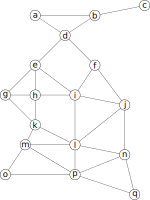
\includegraphics[width=0.7\columnwidth]{8/graph.pdf}
    \caption{{\color{gray} The graph depicting the connectedness of the Wireless Sensor Network under consideration.}}
    \label{fig:8}
\end{figure}

\renewcommand{\labelenumi}{(\alph{enumi})}
\begin{enumerate}
  \item {\color{gray} Suppose 9 frequency channels are available, can the chosen communication protocol be used in the shown network?}
  \item {\color{gray} Determine the minimum number of channels required to be able to use the chosen communication protocol in the shown network.}
  \item {\color{gray} Suppose a different communication protocol requires unique frequency channels in each 3-hop neighborhood instead and 11 channels are available. Determine if this other communication protocol can be used in the shown network. (This means for all nodes $i$, no nodes $j$, $k$ and $l$ with edges $i$-$j$, $j$-$k$ and $k$-$l$ may exist where the channel of $j$, $k$ or $l$ is equal to the channel of $i$.)}
\end{enumerate}

In order to solve this problem an SMT implementation is made which will be detailed below. For each set of two nodes $x$ and $y$ the variables $hop\_1\_x\_y$ and $hop\_1\_y\_x$ are defined. For each pair of nodes that are connected by an edge the constraint is added that the corresponding variables are true, for each pair of nodes that do not share an edge the requirement is added that the corresponding variables are false. This process defines all edges and therefore 1-hop neighbors in the network.

In order to define the $i$-hop neighbors the constraints $hop\_i\_x\_y \implies hop\_{i+1}\_x\_y$ and $hop\_i\_x\_y \vee hop\_1\_y\_z \implies hop\_{i+1}\_x\_z$ are implemented for all possible permutations of the nodes $x$, $y$ and $z$. This process defines the $i$-hop neighbors from the $i-1$-hop neighbors and one extra edge.

\begin{enumerate}
  \item The requirement that the frequency channel should be unique in each 2-hop neighborhood can be expressed by the constraints $hop\_2\_x\_y \implies chan\_x \neq chan\_y$ for all permutations of the nodes $x$ and $y$, while the requirement that only 9 channels are available can be expressed by the constraints $0 \leq chan\_x \leq 8$. Generating the conjunction of all constraints by the Python script listed in \Cref{app:4_gen.py} yields the SMT file listed in \Cref{app:4_a_in}. Running Z3 on this file shows the satisfying assignment listed in \Cref{app:4_a_out} from which it can be concluded that the following channel assignment is a valid assignment:
  \begin{table}[]
    \begin{tabular}{ll|ll}
      Node & Channel & Node & Channel \\ \hline
      A    & 3       & J    & 1       \\
      B    & 6       & K    & 0       \\
      C    & 5       & L    & 3       \\
      D    & 0       & M    & 2       \\
      E    & 5       & N    & 5       \\
      F    & 4       & O    & 4       \\
      G    & 1       & P    & 7       \\
      H    & 7       & Q    & 6       \\
      I    & 8       &      &        
   \end{tabular}
  \end{table}
  This shows that it is indeed possible to use the chosen protocol in the network with 9 channels available.
  \item Changing the requirements regarding the number of channels to $0 \leq chan\_x \leq 6$ and $0 \leq chan\_x \leq 5$ for all nodes $x$ yields the SMT files listed in \Cref{app:4_b1_in} and \Cref{app:4_b2_in} respectively. Running Z3 on these files produces the outputs listed in \Cref{app:4_b1_out} and \Cref{app:4_b2_out} respectively. The fact that the constraints with $0 \leq chan\_x \leq 5$ are unsatisfiable means that there is no way to assign the frequency channels if only 6 channels are available, while for 7 available channels the following assignment is found:
  \begin{table}[]
    \begin{tabular}{ll|ll}
      Node & Channel & Node & Channel \\ \hline
      A    & 1       & J    & 5       \\
      B    & 0       & K    & 4       \\
      C    & 4       & L    & 1       \\
      D    & 2       & M    & 2       \\
      E    & 6       & N    & 6       \\
      F    & 4       & O    & 5       \\
      G    & 5       & P    & 3       \\
      H    & 3       & Q    & 4       \\
      I    & 0       &      &        
   \end{tabular}
  \end{table}
  From this it can be concluded that the minimum number of available channels required is 7.
  \item The constraints concerning the number of available channels can be changed to $0 \leq chan\_x \leq 10$ for all nodes $x$, while the constraints that specify unique channels in a 3-hop neighborhood can be represented by $hop\_3\_x\_y \implies chan\_x \neq chan\_y$ for all permutations of nodes $x$ and $y$. This results in the SMT file listed in \Cref{app:4_c_in}, while running Z3 on this file generates the output listed in \Cref{app:4_c_out}. This output shows that the following channel assignment satisfies all requirements:
  \begin{table}[]
    \begin{tabular}{ll|ll}
      Node & Channel & Node & Channel \\ \hline
      A    & 6       & J    & 4       \\
      B    & 3       & K    & 3       \\
      C    & 4       & L    & 6       \\
      D    & 5       & M    & 5       \\
      E    & 7       & N    & 8       \\
      F    & 0       & O    & 7       \\
      G    & 9       & P    & 10      \\
      H    & 2       & Q    & 9       \\
      I    & 1       &      &        
   \end{tabular}
  \end{table}
  From this it can be concluded that the alternative communication protocol can be used in the network if 11 channels are available.
\end{enumerate}

\onecolumn
\newcommand{\refq}[1]{\texorpdfstring{\Cref{chp:#1}}{q#1}}
\begin{appendices}
\crefalias{chapter}{applbl}

%\chapter{Python script for generating the constraints file for \refq{1}}
%\label{app:1_gen.py}
%\lstinputlisting[language=Python]{1/gen.py}

\end{appendices}

\end{document}
